% ---------------------------------------------------------------
% ---------------------------------------------------------------
% This template was developed for the working paper series of 
% the Interdisciplinary Laboratory of Computational Social Science (iLCSS)
% at the University of Maryland, College Park

% The template was built based on  the PNAS Latex model. 

% Adjustments were made by Tiago Ventura, Ph.D. Student in Political Science at UMD, 
% and researcher at the iLCSS.

\documentclass[9pt,twocolumn,twoside]{ilcss}
\usepackage{listings}
\usepackage[toc,page]{appendix}


\templatetype{ilcssworkingpaper} % Choose template 

\title{Un enfoque bayesiano para el análisis del tiempo de desplazamiento de usuarios del Sistema de Bicicletas Públicas de la Ciudad de México}	

% Use letters for affiliations, numbers to show equal authorship (if applicable) and to indicate the corresponding author
\author[a]{Laura Gómez Bustamante}
\author[a]{Elizabeth Rodríguez Sánchez}
\author[a]{Miguel Ángel Millán Dorado}
\author[a]{C\'esar Zamora Mart\'inez}
%\author[b,1,2]{Author Two} 
%\author[a]{Author Three}

\affil[a]{Alumnos de Maestría en Ciencias de Datos (ITAM)}
%\affil[b]{Affiliation Two}
%\affil[c]{Affiliation Three}

% Please give the surname of the lead author for the running footer
\leadauthor{C\'esar Zamora Mart\'inez} 

% Please add here a significance statement to explain the relevance of your work
%\significancestatement{Authors must submit a 120-word maximum statement about the significance of their research paper written at a level understandable to an undergraduate educated scientist outside their field of speciality. The primary goal of the Significance Statement is to explain the relevance of the work in broad context to a broad readership. The Significance Statement appears in the paper itself and is required for all research papers.}

% Please include corresponding author, author contribution and author declaration information
%\authorcontributions{Please provide details of author contributions here.}
%\authordeclaration{Please declare any conflict of interest here.}
%\equalauthors{\textsuperscript{1}A.O.(Author One) and A.T. (Author Two) contributed equally to this work (remove if not applicable).}
\correspondingauthor{\textsuperscript{2}E-mail: czamora5\@email.itam.mx}

% Keywords are not mandatory, but authors are strongly encouraged to provide them. If provided, please include two to five keywords, separated by the pipe symbol, e.g:
%\keywords{Aprendizaje de Máquina $|$ Banda Ancha $|$ Telecomunicaciones $|$ ITAM} 

\begin{abstract}En fechas recientes el Sistema de Bicicletas Públicas de la Ciudad de México ha ido ganando terreno como una opción de movilidad para la población. Dado que éste cubre diferentes zonas de la ciudad a través de un horario amplio, el tiempo de desplazamiento de sus usuarios obedece a múltiples factores que determinan la actividades diarias que realiza la población.	Motivado por ello, en este trabajo se plantea el análisis de los tiempos de desplazamiento a partir de un enfoque de estadística bayesiana con el propósito de identificar factores que inciden en la duración de los viajes.
\end{abstract}


%\dates{This manuscript was compiled on \today}

% You can change the link on the footer here

%\doi{\url{http://ilcss.umd.edu/}}

\begin{document}

\maketitle
\thispagestyle{firststyle}
\ifthenelse{\boolean{shortarticle}}{\ifthenelse{\boolean{singlecolumn}}{\abscontentformatted}{\abscontent}}{}

% If your first paragraph (i.e. with the \dropcap) contains a list environment (quote, quotation, theorem, definition, enumerate, itemize...), the line after the list may have some extra indentation. If this is the case, add \parshape=0 to the end of the list environment.

\dropcap{D}ada la compleja naturaleza de la movilidad en las ciudades, en tiempos recientes, gobiernos y empresas han notado la importancia de complementar las redes de transporte con medios que permitan satisfacer la demanda de movilidad sobre 1) rutas con características específicas (como zonas de oficinas, centros educativos o lugares de interés turístico), así como 2) tramos que abarcan distancias moderadas.  En tal contexto, las bicicletas han cobrado relevancia como medios que permiten ampliar las capacidades de la infraestructura existente no solo con niveles asequibles de inversión, sino también desde una perspectiva sustentable (véase \cite{Fishman}, \cite{Pojani} y \cite{Stehlin}).

Siguiendo ésta tendencia, a partir de febrero de 2010 se puso en funcionamiento el Sistema de Bicicletas Públicas de la Ciudad de México (Ecobicis), el cual permite a sus usuarios registrados, a través de un esquema de alquiler, tomar una bicicleta de cualquiera de sus estaciones situadas en la vía pública ("cicloestaciones") y devolverla en la más cercana a su destino,  considerando trayectos que en principio no pueden exceder 45 minutos, a menos que el usuario esté dispuesto a pagar una tarifa extra. Los esquemas de renta son flexibles para los usuarios, pues permiten contratar una suscripción que avala el derecho de uso del sistema de Ecobicis, desde un día, tres días, una semana y hasta por un año, con precios que oscilan desde los 104 (plan "Temporal 1 día") hasta 462 pesos mexicanos (plan "Anual")\footnote{Véase https://www.ecobici.cdmx.gob.mx/es/informacion-del-servicio/requisitos-planes-y-tarifas. Al exceder los 45 minutos de uso, se cobran tarifas que van ascendiendo en función del tiempo, desde 13 pesos mexicanos al superar por hasta 15 minutos más el tiempo base, hasta 5,771 pesos mexicanos tras un uso mayor a 24 horas.}.

En términos de cobertura y recursos, tal sistema cuenta, en tiempos actuales, con 480 cicloestaciones repartidas a través de 55 colonias de la ciudad, donde el parque vehicular es cercano a 6,800 bicicletas, las cuales están disponibles para su uso en todo el polígono del sistema, cuya extensión actual abarca 38 $km^2$\footnote{https://www.ecobici.cdmx.gob.mx/es/informacion-del-servicio/que-es-ecobici}.

Por otra parte, de acuerdo a la Encuesta Ecobicis 2017, efectuada por la Secretaría de Movilidad de la Ciudad de México (ver \cite{Ecobicis2017}) los usuarios de Ecobicis emplean los medios de transporte del sistema para actividades relacionadas con su trabajo, viajar a casa, así como por motivos sociales y de ocio.

\section{Revisión y análisis de fuentes de datos asociados a banda ancha fija}

hola

\subsection{Revisión de fuentes de información}

hola
\subsubsection{Identificación de municipios}

hola

\begin{table}[tbhp]
 \centering
	\caption{Distribución de accesos de BAF por tecnología (Junio 2019)\label{table:distribaccesosgrupos}}
	\begin{tabular}{@{}llllll@{}}
		\toprule
		Grupo & Coaxial & DSL & Fibra & Satelital & No especificado \\ \midrule
		América Móvil &  & 71.9\% & 28.1\% &  &  \\ 
		Grupo Televisa & 95.6\% &  &  & 0.1\% & 4.3\% \\ 
		Megacable-MCM & 99.9\% &  &  &  & 0.1\% \\ 
		TotalPlay &  &  & 100\% &  &  \\ \bottomrule
	\end{tabular}
\end{table}


\subsection{Conclusiones}

En este documento, exploramos el uso de modelos 
\bibliography{ilcss-sample}

\begin{appendices}
	
	\section{Repositorio Github}
	
	El desarrollo de este trabajo se consolidó a través de un repositorio en Github de acceso público: https://github.com/czammar/BandaAnchaFija; este contiene la totalidad de script desarrollados en Bash, R, Python, los mapas interactivos, las versiones en .tex de los documentos así como los datos empleados.
	
	\section{Figuras de análisis exploratorio}

\begin{figure}[tbhp]
	\centering
	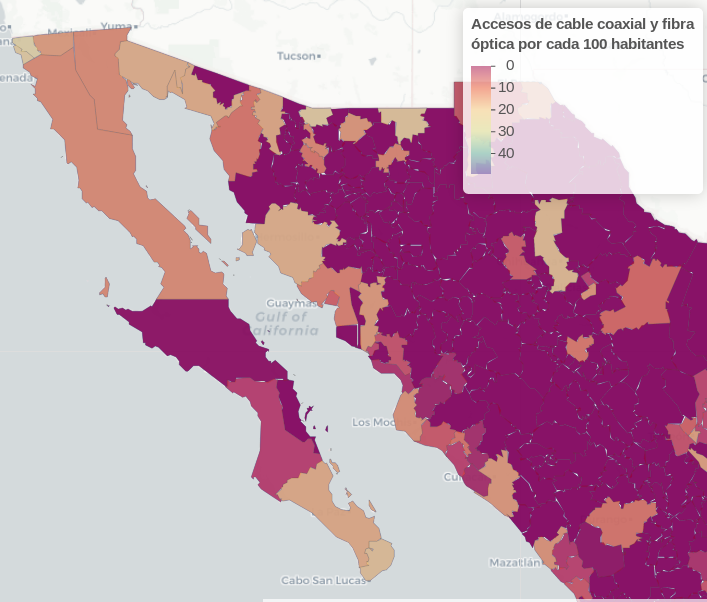
\includegraphics[width=0.9\linewidth]{images/pen_habs_penbc.png}
	\caption{Penetración de cable coaxial y fibra en la península de Baja California}
	\label{fig:pen_habs_penbc}
\end{figure}
\end{appendices}

\end{document}